% Provenance (never printed): cycle 4 SVT, "La planete Terre": sedimentation,
% from sediment to sedimentary rock, fossilisation, fossils and layers as a
% record of past environments; see sources/book1/PROVENANCE.md. Book 1,
% grade 7, chapter 4.
% Vocabulary guard: first chapter allowed to use "sediment"; the principles of
% relative dating (superposition, fossil succession and the rest) and "unconformity" are
% g7.5's and are not named here; fossils as evidence of evolution are the
% biology books' (one sentence of prose).
\chapter{沉积物与化石}\label{ch:g7:sediments-and-fossils}

大峡谷位于美国亚利桑那州，平均深度为
\qty{1.6}{km}。岩壁由一层叠一层的\omterm{def:g3:stones-pebbles-sand:rock}{岩石}构成，
颜色有红色、棕色、灰色和乳白色。
最上层的凯巴布石灰岩中，护林员指给人看贝壳——腕足动物的壳，
这种动物曾生活在海底。
这块\omterm{def:g3:stones-pebbles-sand:rock}{岩石}形成于\omterm{def:g2:water-on-earth:ocean}{海洋}底部，如今构成峡谷的边缘，远高于\omterm{def:g4:world-physical-map:altitude}{海平面}。
% ledger: nps:grca-depth, nps:grca-fossils, nps:grca-kaibab

\begin{omfigure}
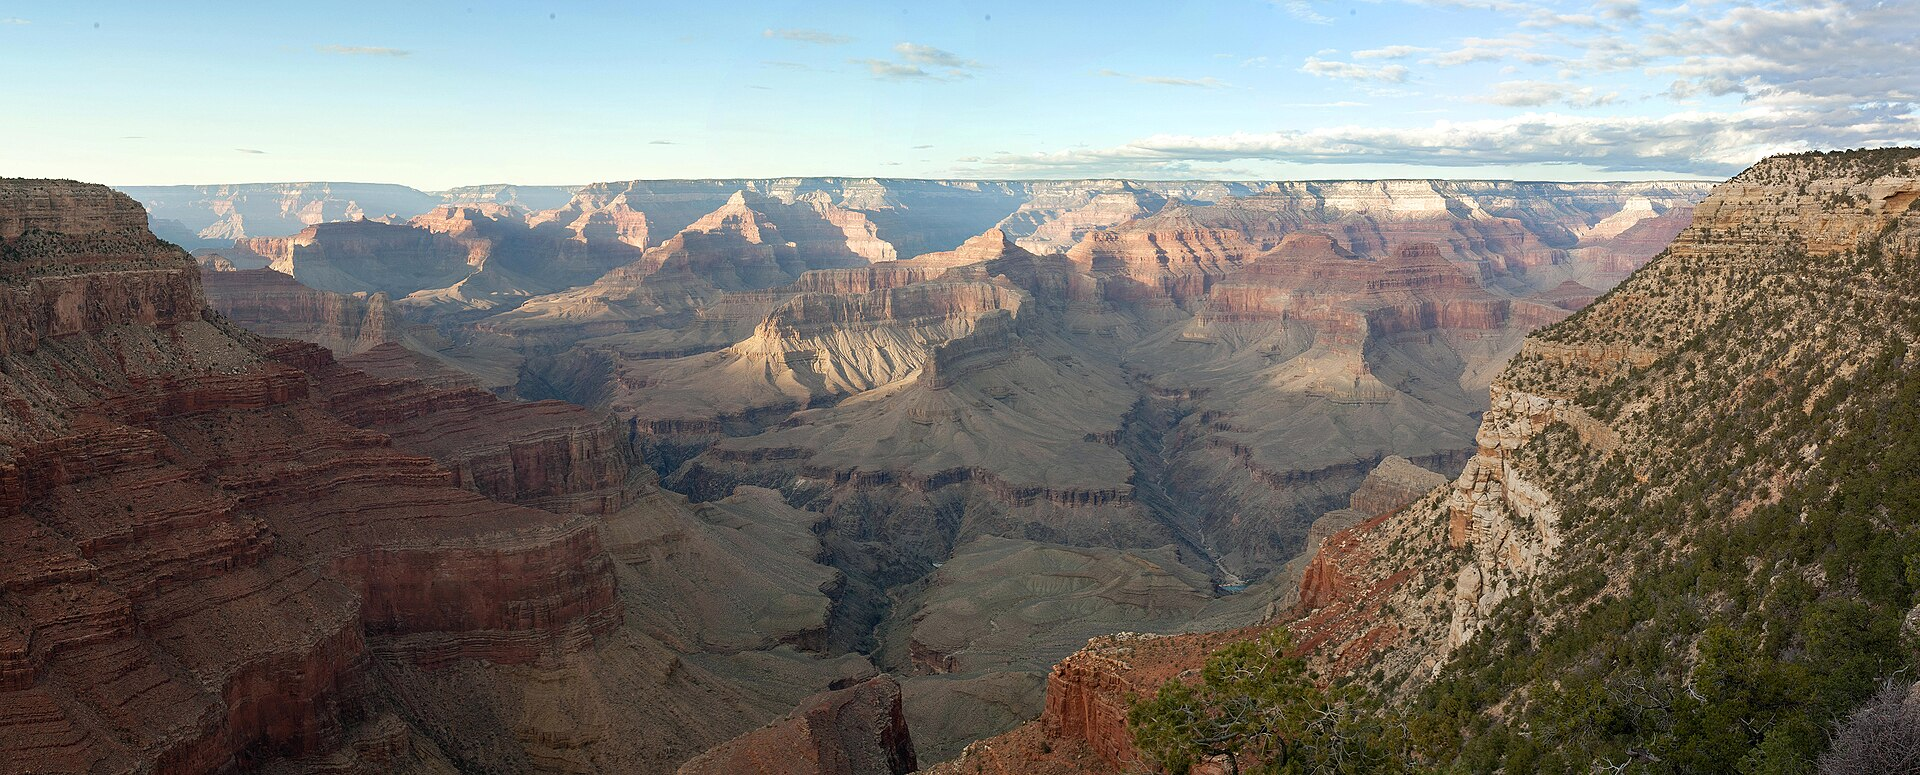
\includegraphics[width=\linewidth]{images/book1/g7-grand-canyon.jpg}

{\small 从南缘的赫米特休息点望去的大峡谷：岩层一层叠一层，
自峡谷边缘直至谷底。NPS 照片，摄影：Kristen M. Caldon。
（公有领域，经由维基共享资源）。}
% ledger: commons:grand-canyon
\label{fig:g7:sediments-and-fossils:canyon}
\end{omfigure}

松散的沙和泥怎样变成坚硬的\omterm{def:g3:stones-pebbles-sand:rock}{岩石}？
一个贝壳怎样保存如此之久，最终被包在悬崖之中？
而\omterm{def:g7:sediments-and-fossils:layer}{地层}与\omterm{def:g7:sediments-and-fossils:fossil}{化石}又能告诉我们，很久以前的地方是什么样子？

\begin{recall}
\omterm{def:g3:stones-pebbles-sand:rock}{岩石}在地表缓慢地破碎成碎块（\emph{\omterm{def:g5:water-shapes-the-land:weathering}{风化}}）；
水、风和冰把碎块搬走（\emph{\omterm{def:g5:water-shapes-the-land:erosion}{侵蚀}}），
并在它们减速、停止的地方堆积下来（\emph{\omterm{def:g5:water-shapes-the-land:deposition}{沉积}}）：最重的先沉，
细泥只在水几乎静止的地方才沉下来
（\cref{ch:g5:water-shapes-the-land}）。\emph{\omterm{def:g6:rocks-and-minerals:rock-families}{沉积岩}}形成于地表，
由\omterm{def:g3:stones-pebbles-sand:sand}{沙粒}、泥或贝壳分层堆积并固结而成，
如砂岩、页岩和石灰岩。\omterm{def:g6:rocks-and-minerals:rock-cycle}{岩石循环}
使各类\omterm{def:g3:stones-pebbles-sand:rock}{岩石}之间缓慢地相互转化
（\cref{ch:g6:rocks-and-minerals}）。
\end{recall}

\section{沉积物成层沉降}

只要水、风或冰把所携带的物质放下，
就会积聚起松散的\omterm{def:g7:sediments-and-fossils:sediment}{沉积物}：河床上的\omterm{def:g3:stones-pebbles-sand:pebble}{砾石}和沙、湖底的泥，
海滩或沙丘上的沙，以及海底的贝壳。

\begin{definition}[沉积物]\label{def:g7:sediments-and-fossils:sediment}
称\emph{沉积物}\index{沉积物}为由水、风或冰堆积下来的松散物质，
包括\omterm{def:g3:stones-pebbles-sand:pebble}{砾石}、沙、泥，以及生物的壳和骨骼。
它堆积于\omterm{def:g1:landscapes-around-us:water}{河流}、\omterm{def:g1:landscapes-around-us:water}{湖泊}和\omterm{def:g2:water-on-earth:ocean}{海洋}底部，
也堆积于风或冰将其留下的陆地上。
\end{definition}

\omterm{def:g7:sediments-and-fossils:sediment}{沉积物}按一定的顺序沉降。浑水变慢时，
最大、最重的颗粒先下沉，最细、最轻的颗粒
最后下沉。水流每次发生变化——一场\omterm{def:g5:water-shapes-the-land:flood}{洪水}带来沙，接着是只有细泥到达底部的平静数周——
沉降的颗粒随之改变，
又开始形成新的一层。日积月累，湖底或海底
被一叠\omterm{def:g7:sediments-and-fossils:layer}{沉积层}覆盖，最老的一层位于
这叠的最底部。
% ledger: usgs:strata, usgs:sediments-to-rock

\begin{omfigure}
\begin{tikzpicture}[font=\small, x=1cm, y=1cm]
  % land and river
  \fill[omLithAlluv] (0,3.0) -- (2.0,2.45) -- (2.0,0) -- (0,0) -- cycle;
  \fill[blue!35] (0,3.05) -- (2.0,2.5) -- (2.0,2.4) -- (0,2.95) -- cycle;
  % lake water
  \fill[omSea!45] (2.0,2.5) -- (12.4,2.5) -- (12.4,1.12) -- (3.0,1.2) -- cycle;
  \draw[blue!50!black, line width=0.6pt] (2.0,2.5) -- (12.4,2.5);
  % layers on the bottom: thick near the mouth, thinner far out
  \foreach \k/\c in {0/omLithSand, 1/omLithShale, 2/omLithSand, 3/omLithShale} {
    \pgfmathsetmacro{\yb}{0.2+0.25*\k}
    \pgfmathsetmacro{\yt}{0.2+0.25*(\k+1)}
    \fill[\c] (3.0,\yb) -- (12.4,\yb) -- (12.4,\yt-0.08) -- (3.0,\yt) -- cycle;
  }
  \draw[black!60, line width=0.3pt] (3.0,1.2) -- (12.4,1.12);
  \fill[omLithAlluv!80!black] (2.0,0) rectangle (12.4,0.2);
  \fill[omLithAlluv] (2.0,0.2) -- (3.0,0.2) -- (3.0,1.2) -- (2.0,2.45) -- cycle;
  % settling grains: big ones near the mouth, fine ones far out
  \foreach \x/\y in {3.3/2.1, 3.6/1.75, 3.9/2.25, 4.2/1.55, 3.5/1.35, 4.5/2.0} {
    \fill[brown!70!black] (\x,\y) circle (0.07);
    \draw[-{Stealth[length=1.3mm]}, black!60] (\x,\y-0.1) -- (\x,\y-0.32);
  }
  \foreach \x/\y in {6.5/2.2, 7.4/1.8, 8.3/2.15, 9.1/1.6, 9.9/2.05, 10.8/1.75, 11.6/2.1, 7.9/1.35, 10.4/1.3} {
    \fill[brown!50!black] (\x,\y) circle (0.025);
    \draw[-{Stealth[length=1mm]}, black!40] (\x,\y-0.05) -- (\x,\y-0.2);
  }
  \node[anchor=south, align=center] at (1.0,3.1) {洪水期的河流 \\[-2pt]带来沙和泥};
  \node[anchor=south, align=center] at (4.1,2.55) {沙先沉降，\\[-2pt]靠近河口};
  \node[anchor=south, align=center] at (9.2,2.55) {细泥缓慢沉降，\\[-2pt]在远处水流平静之处};
  \draw[decorate, decoration={brace, amplitude=4pt}] (12.55,1.15) -- (12.55,0.2)
    node[midway, anchor=west, xshift=4pt, align=left, font=\footnotesize] {湖底的沉积层：\\[-2pt]沙、泥、沙、泥};
\end{tikzpicture}

{\small \omterm{def:g7:sediments-and-fossils:sediment}{沉积物}在湖中沉降（示意图，不按比例绘制）。每次
\omterm{def:g5:water-shapes-the-land:flood}{洪水}之后先沉下一层沙，随后是平静数周内沉下的细泥：
层层堆积，于湖底形成\omterm{def:g7:sediments-and-fossils:layer}{沉积层}。}
% ledger: usgs:strata
\label{fig:g7:sediments-and-fossils:lake}
\end{omfigure}

\begin{definition}[沉积层]\label{def:g7:sediments-and-fossils:layer}
称\emph{沉积层}\index{沉积层}，或
\emph{地层}\index{地层}（复数 \emph{strata}）是一层
\omterm{def:g7:sediments-and-fossils:sediment}{沉积物}或其所形成的\omterm{def:g3:stones-pebbles-sand:rock}{岩石}，在同一时期\omterm{def:g5:water-shapes-the-land:deposition}{沉积}下来。它具有
底面和顶面，其与上下相邻的层
在颗粒大小或组成物质上有所不同。
\end{definition}

\omterm{def:g7:sediments-and-fossils:sediment}{沉积物}从水中或空气中沉降，因此呈水平状堆积，
就像平放在桌上的书页。若发现\omterm{def:g7:sediments-and-fossils:layer}{地层}倾斜或
褶皱，说明它们形成之后曾受到外力移动。层理是
\omterm{def:g6:rocks-and-minerals:rock-families}{沉积岩}最明显的标志：你在大峡谷的崖壁上就见过它。
% ledger: usgs:strata, nps:grca-kaibab

\begin{inthelab}[罐中的地层（课堂上，在教师指导下进行）]
在一个高玻璃罐中放入一把\omterm{def:g3:stones-pebbles-sand:pebble}{砾石}、两把沙和几勺土壤；
注入水，盖紧盖子后摇匀。
放下静置几分钟，观察：\omterm{def:g3:stones-pebbles-sand:pebble}{砾石}几乎立即沉到罐底，
沙稍晚一些沉降，而细泥则使水长时间保持浑浊，
可达数小时。次日，再加入少量土壤和沙，轻轻摇动，
并使其再次沉降。你能数出几层吗？每层的底部
分别是什么颗粒？
\end{inthelab}

\section{从沉积物到岩石}

一层\omterm{def:g7:sediments-and-fossils:sediment}{沉积物}不会长久留在表面。其上相继\omterm{def:g5:water-shapes-the-land:deposition}{沉积}新的
\omterm{def:g7:sediments-and-fossils:layer}{地层}，它被埋得越来越深。在上覆\omterm{def:g7:sediments-and-fossils:layer}{地层}的
重压之下，颗粒被挤得更紧密，颗粒间的水被挤出。
渗流穿过\omterm{def:g7:sediments-and-fossils:layer}{沉积层}的水会在颗粒之间留下
\omterm{def:g6:rocks-and-minerals:mineral}{矿物}，这种天然胶结物将颗粒粘连在一起，
经过长时间，随着\omterm{def:g7:sediments-and-fossils:layer}{地层}不断堆积，并伴随缓慢的化学
变化，堆积底部的松散\omterm{def:g7:sediments-and-fossils:sediment}{沉积物}变成了\omterm{def:g3:stones-pebbles-sand:rock}{岩石}。
% ledger: usgs:sediments-to-rock, usgs:sedimentary

每种\omterm{def:g7:sediments-and-fossils:sediment}{沉积物}形成各自的\omterm{def:g3:stones-pebbles-sand:rock}{岩石}。

\begin{center}
\small
\begin{tabular}{|l|l|}
\hline
\textbf{\omterm{def:g7:sediments-and-fossils:sediment}{沉积物}} & \textbf{形成的\omterm{def:g3:stones-pebbles-sand:rock}{岩石}} \\
\hline
\omterm{def:g3:stones-pebbles-sand:pebble}{砾石}和\omterm{def:g3:stones-pebbles-sand:pebble}{卵石} & 砾岩 \\
沙 & 砂岩 \\
泥 & 泥岩，若能裂分成薄片则为页岩 \\
贝壳和骨骼 & 石灰岩 \\
埋藏于沼泽中的植物遗体 & 煤 \\
\hline
\end{tabular}
\end{center}
% ledger: usgs:sediments-to-rock, usgs:sedimentary, usgs:coal-origin

\begin{omfigure}
\begin{tikzpicture}[font=\small, x=1cm, y=1cm]
  \pgfmathsetseed{11}
  \foreach \p/\gap/\title in {0/0.40/{松散的沉积物}, 1/0.31/{被埋藏、受挤压：\\[-2pt]水被挤出}, 2/0.31/{被胶结：成为岩石}} {
    \begin{scope}[xshift=\p*4.6cm]
      \ifnum\p=2 \fill[black!25] (0,0) rectangle (3.4,3.0);
      \else \fill[omSea!45] (0,0) rectangle (3.4,3.0); \fi
      \foreach \i in {0,...,7} {
        \foreach \j in {0,...,6} {
          \pgfmathsetmacro{\gx}{0.25 + \i*\gap*1.05 + 0.05*rand}
          \pgfmathsetmacro{\gy}{0.25 + \j*\gap + 0.05*rand}
          \pgfmathsetmacro{\gr}{0.13 + 0.03*rand}
          \ifdim\gx pt<3.25pt \ifdim\gy pt<2.85pt
            \fill[omLithSand!80!brown, draw=brown!60!black, line width=0.3pt] (\gx,\gy) circle (\gr);
          \fi\fi
        }
      }
      \draw[black!70, line width=0.6pt] (0,0) rectangle (3.4,3.0);
      \node[anchor=north, align=center] at (1.7,-0.1) {\title};
    \end{scope}
  }
  \draw[-{Stealth[length=2.5mm]}, line width=1pt] (3.6,1.5) -- (4.4,1.5);
  \draw[-{Stealth[length=2.5mm]}, line width=1pt] (8.2,1.5) -- (9.0,1.5);
  \foreach \x in {5.3,6.3,7.3} \draw[-{Stealth[length=2mm]}, line width=0.8pt] (\x,3.7) -- (\x,3.1);
  \node[anchor=south] at (6.3,3.7) {上覆地层的重量};
  \node[anchor=south, font=\footnotesize, align=center] at (10.9,3.05) {灰色：天然胶结物};
\end{tikzpicture}

{\small 从沙到砂岩（颗粒示意图，大幅放大）。
左：颗粒松散，颗粒之间有水。中：埋入新\omterm{def:g7:sediments-and-fossils:layer}{地层}之下，
颗粒被压紧。右：水留下的\omterm{def:g6:rocks-and-minerals:mineral}{矿物}
将颗粒胶结在一起。}
% ledger: usgs:sediments-to-rock, usgs:sedimentary
\label{fig:g7:sediments-and-fossils:to-rock}
\end{omfigure}

你能在地表看到的大多数\omterm{def:g3:stones-pebbles-sand:rock}{岩石}都是
\omterm{def:g6:rocks-and-minerals:rock-families}{沉积岩}。它们形成的\omterm{def:g7:sediments-and-fossils:layer}{地层}堆积，就是
该地方的“历史书”：每一层是一页，最老的一页在最底下。
% ledger: usgs:sediments-to-rock

\section{化石是如何形成的}

\begin{definition}[化石]\label{def:g7:sediments-and-fossils:fossil}
称\emph{化石}\index{化石}，是保存在\omterm{def:g3:stones-pebbles-sand:rock}{岩石}中的古代生物
遗体或遗迹。有些化石保留了生物坚硬的部分，如贝壳、
骨骼、牙齿、木材，它们经石化而形成。另一些化石只保留
形状：\emph{外模}\index{外模}是贝壳或骨骼溶解后在\omterm{def:g3:stones-pebbles-sand:rock}{岩石}中
留下的空穴印痕；\emph{内模}\index{内模}是外模被新的\omterm{def:g6:rocks-and-minerals:mineral}{矿物}质
或\omterm{def:g7:sediments-and-fossils:sediment}{沉积物}充填后形成的复制品。\emph{遗迹化石}\index{遗迹化石}
是动物活动留下的痕迹，如足迹、洞穴、爬痕，
而非动物身体的
一部分。
\end{definition}

\omterm{def:g7:sediments-and-fossils:fossil}{化石}的形成始于动物或植物死后落到
海或湖的底部。若遗体未被掩埋，细菌会将其分解，
水也会慢慢溶解残留物。只有在被迅速掩埋、
被\omterm{def:g7:sediments-and-fossils:sediment}{沉积物}覆盖并隔绝之后，才有机会保存下来。
随后，\omterm{def:g7:sediments-and-fossils:sediment}{沉积物}转变为\omterm{def:g3:stones-pebbles-sand:rock}{岩石}，渗入\omterm{def:g7:sediments-and-fossils:layer}{地层}的水
带来\omterm{def:g6:rocks-and-minerals:mineral}{矿物}，填满贝壳或骨骼的每一个细小\omterm{def:g6:water-underground:porosity}{孔隙}，
使其变成石头。很久以后，上覆\omterm{def:g7:sediments-and-fossils:layer}{地层}可能被\omterm{def:g5:water-shapes-the-land:erosion}{侵蚀}掉，
\omterm{def:g7:sediments-and-fossils:fossil}{化石}便出现在地表。
% ledger: ucmp:fossil-conditions, ucmp:fossil-kinds, usgs:sediments-to-rock

\begin{omfigure}
\begin{tikzpicture}[font=\small, x=0.86cm, y=0.86cm,
    shell/.pic={
      \fill[#1] (0,0) circle (0.42);
      \draw[brown!40!black, line width=0.5pt] plot[domain=0:12.5, samples=90, smooth]
        ({0.032*\x*cos(\x r)}, {0.032*\x*sin(\x r)});
      \draw[brown!40!black, line width=0.5pt] (0,0) circle (0.42);
    }]
  % 1: death on the sea floor
  \begin{scope}[xshift=0cm]
    \fill[omSea!45] (0,1.2) rectangle (3.3,3.6);
    \fill[omLithShale] (0,0) rectangle (3.3,1.2);
    \pic at (1.65,1.62) {shell=omLithSand!60!white};
    \node[anchor=north, align=center] at (1.65,-0.1) {1. 死于 \\[-2pt]海底};
  \end{scope}
  % 2: quick burial
  \begin{scope}[xshift=3.75cm]
    \fill[omSea!45] (0,2.1) rectangle (3.3,3.6);
    \fill[omLithShale] (0,0) rectangle (3.3,1.2);
    \fill[omLithShale!70!white] (0,1.2) rectangle (3.3,2.1);
    \pic at (1.65,1.62) {shell=omLithSand!60!white};
    \foreach \x in {0.5,1.2,2.1,2.8} \fill[brown!50!black] (\x,2.4) circle (0.03);
    \node[anchor=north, align=center] at (1.65,-0.1) {2. 泥沙 \\[-2pt]迅速掩埋};
  \end{scope}
  % 3: buried deep, turned to stone
  \begin{scope}[xshift=7.5cm]
    \fill[omLithShale!80!black] (0,0) rectangle (3.3,1.2);
    \fill[omLithShale!85!black] (0,1.2) rectangle (3.3,2.1);
    \fill[omLithSand] (0,2.1) rectangle (3.3,2.9);
    \fill[omLithLime] (0,2.9) rectangle (3.3,3.6);
    \pic at (1.65,1.62) {shell=black!35};
    \node[anchor=north, align=center] at (1.65,-0.1) {3. 深埋后，\\[-2pt]变为石头};
  \end{scope}
  % 4: uncovered by erosion
  \begin{scope}[xshift=11.25cm]
    \fill[white] (0,0) rectangle (3.3,3.6);
    \fill[omLithShale!80!black] (0,0) -- (3.3,0) -- (3.3,2.6) -- (2.4,2.3) -- (1.8,1.95) -- (1.2,1.7) -- (0,1.5) -- cycle;
    \draw[black!35, line width=0.4pt] (0,1.2) -- (3.3,1.2);
    \draw[black!60, line width=0.4pt] (0,1.5) -- (1.2,1.7) -- (1.8,1.95) -- (2.4,2.3) -- (3.3,2.6);
    \pic at (1.65,1.84) {shell=black!35};
    \node[anchor=north, align=center] at (1.65,-0.1) {4. 侵蚀使其 \\[-2pt]露出地表};
  \end{scope}
  \foreach \p in {0,1,2,3} {
    \begin{scope}[xshift=\p*3.75cm]
      \draw[black!70, line width=0.5pt] (0,0) rectangle (3.3,3.6);
    \end{scope}
  }
\end{tikzpicture}

{\small \omterm{def:g7:sediments-and-fossils:fossil}{化石}形成过程（示意图，未按比例）：贝壳被
\omterm{def:g3:stones-pebbles-sand:sand}{泥沙}迅速掩埋；深埋于新\omterm{def:g5:water-shapes-the-land:deposition}{沉积}的\omterm{def:g7:sediments-and-fossils:layer}{地层}之下后，变为石头；
很久以后，\omterm{def:g5:water-shapes-the-land:erosion}{侵蚀}作用剥去上覆\omterm{def:g7:sediments-and-fossils:layer}{地层}，\omterm{def:g7:sediments-and-fossils:fossil}{化石}
出露于地表。}
% ledger: ucmp:fossil-conditions, ucmp:fossil-kinds
\label{fig:g7:sediments-and-fossils:steps}
\end{omfigure}

大多数生物根本不会留下\omterm{def:g7:sediments-and-fossils:fossil}{化石}。软体在被掩埋前就已腐烂，
即使是贝壳和骨骼，若长期暴露在外，也会破碎或溶解。
\omterm{def:g7:sediments-and-fossils:fossil}{化石}最易形成的地方，是安静的海或湖的底部，
细软的\omterm{def:g3:stones-pebbles-sand:sand}{泥沙}在遗体上\omterm{def:g5:water-shapes-the-land:deposition}{沉积}，将其保护起来。
因此，\omterm{def:g3:stones-pebbles-sand:rock}{岩石}中发现的\omterm{def:g7:sediments-and-fossils:fossil}{化石}大多是贝壳，
以及微小贝壳和微观动植物的遗骸；恐龙
虽是最著名的\omterm{def:g7:sediments-and-fossils:fossil}{化石}，却只占其中很小的一部分。
% ledger: ucmp:fossil-conditions, usgs:fossil-record-shells

\begin{omfigure}
\begin{minipage}[t]{0.49\linewidth}\centering
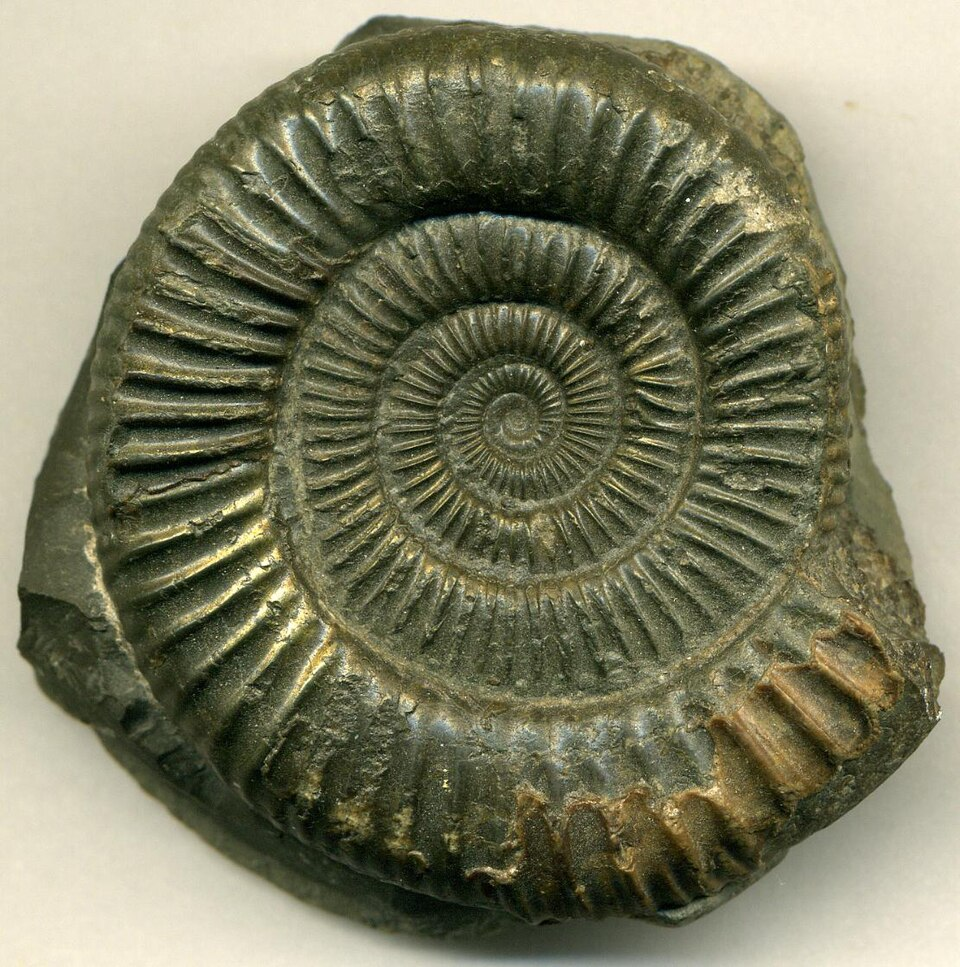
\includegraphics[height=4.6cm]{images/book1/g7-ammonite.jpg}

{\small 菊石，一种已灭绝的动物，贝壳呈螺旋形，是鱿鱼和章鱼的
亲属，直径\qty{5.7}{cm}，产自
英格兰约克郡\omterm{def:g1:landscapes-around-us:water}{海岸}。}
\end{minipage}\hfill
\begin{minipage}[t]{0.49\linewidth}\centering
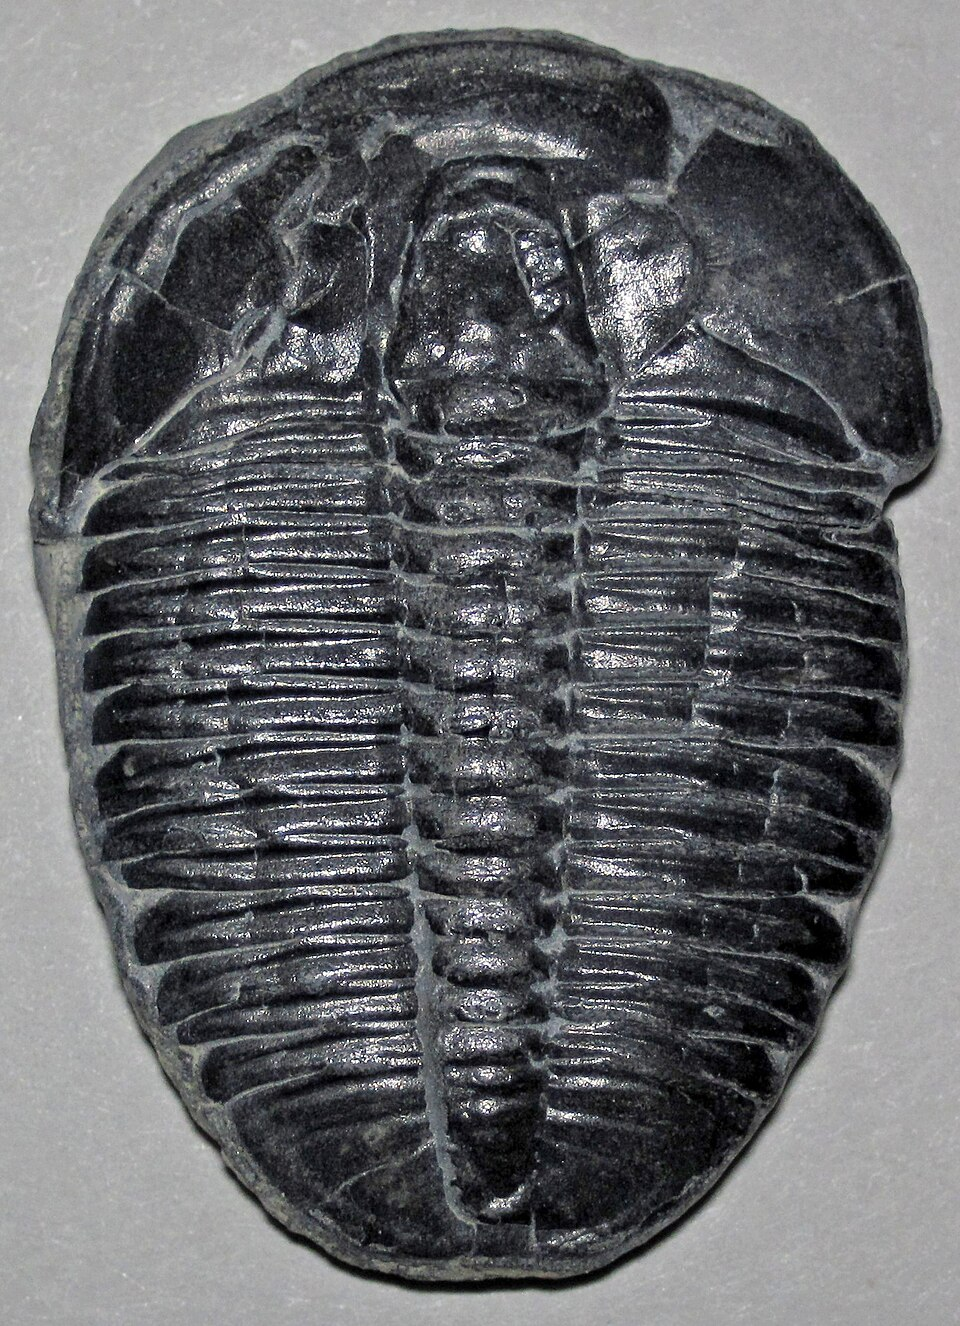
\includegraphics[height=4.6cm]{images/book1/g7-trilobite.jpg}

{\small 三叶虫，一种已灭绝的\omterm{def:g2:water-on-earth:ocean}{海洋}动物，身体分为三叶，
直径约\qty{2.6}{cm}，产自美国犹他州。}
\end{minipage}\par\medskip

{\small 两件带硬壳的动物\omterm{def:g7:sediments-and-fossils:fossil}{化石}。照片：James
St.~John（CC BY 2.0，经由维基共享资源）。}
% ledger: commons:ammonite, commons:trilobite, nps:ammonoid, nps:trilobite
\label{fig:g7:sediments-and-fossils:ammonite-trilobite}
\end{omfigure}

有时贝壳本身并不会保存下来。被埋在沙中后，
它会被渗过\omterm{def:g3:stones-pebbles-sand:sand}{沙粒}的水慢慢溶解，只留下一个空腔，
空腔内壁印有贝壳的形状，这就是\omterm{def:g7:sediments-and-fossils:fossil}{外模}。若
之后\omterm{def:g6:rocks-and-minerals:mineral}{矿物}\omterm{def:g5:water-shapes-the-land:deposition}{沉积}于空腔中并将其充满，便形成贝壳的复制品，
即\omterm{def:g7:sediments-and-fossils:fossil}{内模}。
% ledger: ucmp:casts-molds

\begin{omfigure}
\begin{tikzpicture}[font=\small, x=1cm, y=1cm,
    clam/.style={line width=0.5pt}]
  \foreach \p/\fillc/\title in {0/{omLithSand!50!white}/{埋在沙中的\\[-2pt]贝壳}, 1/{white}/{贝壳已溶解：\\[-2pt]形成外模}, 2/{black!40}/{矿物充填外模：\\[-2pt]形成内模}} {
    \begin{scope}[xshift=\p*4.9cm]
      \fill[omLithSand] (0,0) rectangle (4.2,2.6);
      \foreach \i in {0,...,40} {
        \pgfmathsetmacro{\gx}{0.1+mod(\i*0.53,4.0)}
        \pgfmathsetmacro{\gy}{0.1+mod(\i*0.37,2.4)}
        \fill[brown!60!black] (\gx,\gy) circle (0.025);
      }
      \fill[\fillc, draw=brown!40!black, clam] (0.9,0.9) arc[start angle=180, end angle=0, x radius=1.2, y radius=0.95] -- cycle;
      \ifnum\p=1
        \foreach \a in {25,45,...,155} \draw[brown!50!black, line width=0.4pt] (2.1,0.9) -- ++(\a:0.93 and 0.75);
      \else
        \foreach \a in {25,45,...,155} \draw[brown!40!black, line width=0.4pt] (2.1,0.9) -- ++(\a:1.05 and 0.85);
      \fi
      \draw[black!70, line width=0.5pt] (0,0) rectangle (4.2,2.6);
      \node[anchor=north, align=center] at (2.1,-0.1) {\title};
    \end{scope}
  }
  \draw[-{Stealth[length=2.5mm]}, line width=1pt] (4.3,1.3) -- (4.8,1.3);
  \draw[-{Stealth[length=2.5mm]}, line width=1pt] (9.2,1.3) -- (9.7,1.3);
\end{tikzpicture}

{\small \omterm{def:g7:sediments-and-fossils:fossil}{外模}与\omterm{def:g7:sediments-and-fossils:fossil}{内模}（\omterm{def:g3:stones-pebbles-sand:rock}{岩石}切开后的示意图）。
\omterm{def:g7:sediments-and-fossils:fossil}{外模}是空腔，壁上印有贝壳的肋纹；
\omterm{def:g7:sediments-and-fossils:fossil}{内模}是贝壳的石质复制品，由充填其中的\omterm{def:g6:rocks-and-minerals:mineral}{矿物}构成。}
% ledger: ucmp:casts-molds
\label{fig:g7:sediments-and-fossils:mould-cast}
\end{omfigure}

动物也会留下其活动的\omterm{def:g7:sediments-and-fossils:fossil}{化石}。一只动物在
河岸或\omterm{def:g1:landscapes-around-us:water}{海岸}松软湿润的泥地上行走，会留下足迹。多数
足迹会被下一次波浪或\omterm{def:g5:water-shapes-the-land:flood}{洪水}冲走。但若\omterm{def:g3:stones-pebbles-sand:sand}{沙子}在
足迹被抹去前将其覆盖，足迹便被填满，\omterm{def:g3:stones-pebbles-sand:sand}{沙子}随后变为砂岩；
\omterm{def:g3:stones-pebbles-sand:rock}{岩石}沿层面裂开时，一侧显露出足迹，
另一侧则为足迹的\omterm{def:g7:sediments-and-fossils:fossil}{内模}。
% ledger: ucmp:footprints

\begin{omfigure}
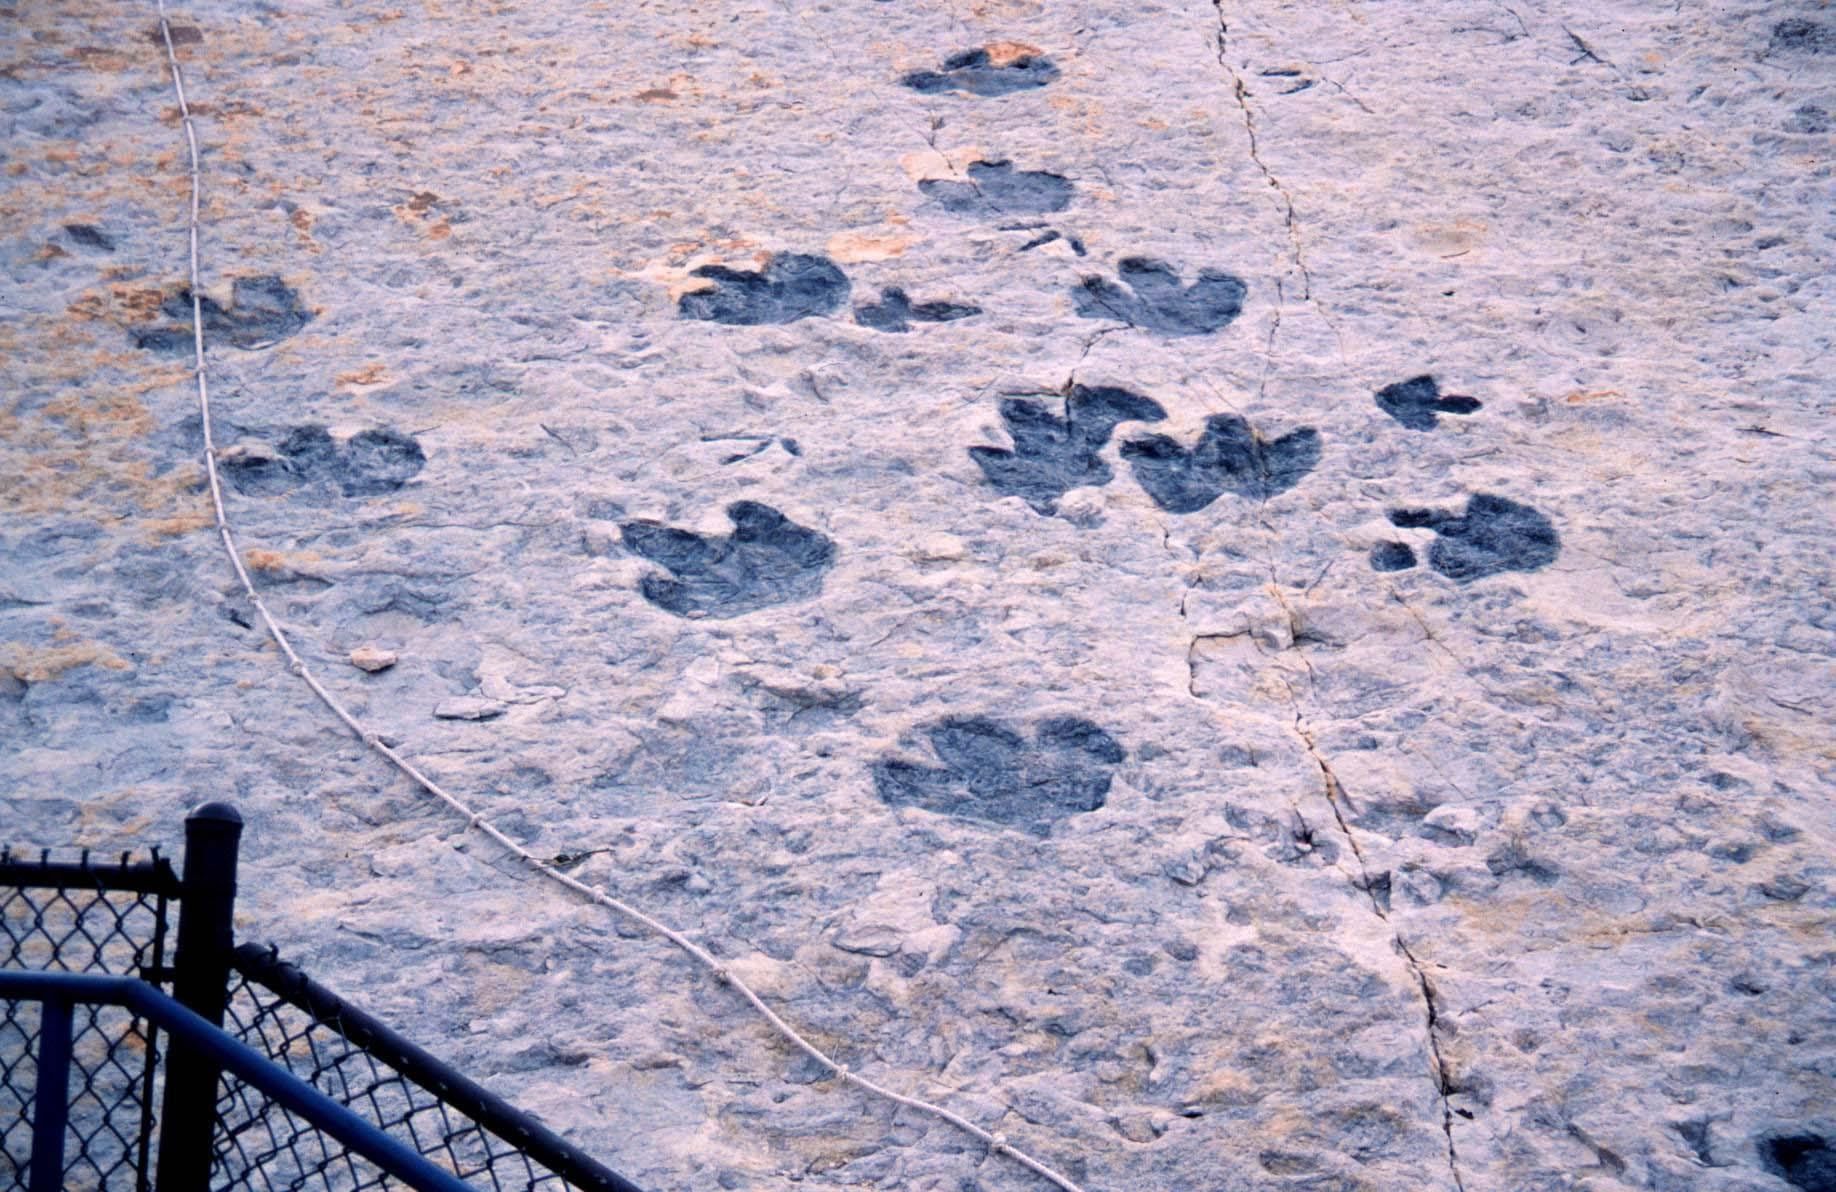
\includegraphics[width=0.62\linewidth]{images/book1/g7-dinosaur-tracks.jpg}

{\small 恐龙足迹，位于科罗拉多州莫里森附近的恐龙岭
（美国）：数十个足迹留在松软的地面上，如今成为倾斜的
\omterm{def:g3:stones-pebbles-sand:rock}{岩石}表面。多数由食草恐龙留下，少数由
细趾的食肉恐龙留下。照片：Dexter Perkins（CC0，经
维基共享资源）。}
% ledger: commons:dino-tracks
\label{fig:g7:sediments-and-fossils:tracks}
\end{omfigure}

生物学借助\omterm{def:g7:sediments-and-fossils:fossil}{化石}追溯生物的漫长历史。在
本书中，\omterm{def:g7:sediments-and-fossils:fossil}{化石}是另一类线索：它们告诉我们
动物生活时那里是什么样子。

\section{地层与化石：过去的记录}

每一层都保留着\omterm{def:g5:water-shapes-the-land:deposition}{沉积}时所在地点的痕迹。珊瑚
礁今日生长于温暖、清澈的浅海中；波痕形成于
浅水之中、\omterm{def:g1:landscapes-around-us:water}{湖泊}、\omterm{def:g1:landscapes-around-us:water}{河流}或\omterm{def:g2:water-on-earth:ocean}{海洋}边缘的沙上；煤形成于
古老森林与沼泽中的植物；腕足动物、海百合
和三叶虫只生活在海中。若在古老岩层中发现相同线索，
则该层形成时的环境很可能与此相似。
% ledger: noaa:coral-where, nps:ripple-marks, nps:ripples-shallow, usgs:coal-origin, nps:trilobite

\begin{center}
\small
\begin{tabular}{|p{0.36\linewidth}|p{0.52\linewidth}|}
\hline
\textbf{岩层中的线索} & \textbf{岩层形成时的地点} \\
\hline
珊瑚 & 温暖、清澈的浅海 \\
\hline
\omterm{def:g2:water-on-earth:ocean}{海洋}动物的壳（腕足动物、海百合、三叶虫） & 海 \\
\hline
岩层表面的波痕 & 浅水，位于湖、河或海的边缘 \\
\hline
足迹 & 松软湿润的泥或沙，常位于\omterm{def:g1:landscapes-around-us:water}{海岸}或河岸 \\
\hline
煤 & 沼泽森林或沼泽 \\
\hline
叶与蜻蜓翅膀 & 陆地，有植物生长 \\
\hline
\end{tabular}
\end{center}
% ledger: noaa:coral-where, nps:grca-fossils, nps:trilobite, nps:ripple-marks, nps:ripples-shallow, ucmp:footprints, usgs:coal-origin

\begin{method}[读取岩层]\label{met:g7:sediments-and-fossils:reading}
\begin{enumerate}
  \item 观察颗粒：粗颗粒\omterm{def:g5:water-shapes-the-land:deposition}{沉积}于水流湍急处，
        细泥只\omterm{def:g5:water-shapes-the-land:deposition}{沉积}于水流平静处。
  \item 寻找\omterm{def:g7:sediments-and-fossils:fossil}{化石}和痕迹（珊瑚、贝壳、足迹、波痕、
        植物遗体、煤），并利用上表。
  \item 将线索综合起来，形成对该地点的整体图景：陆地或
        \omterm{def:g2:water-on-earth:ocean}{海洋}；浅水或深水；平静或流动的水。
\end{enumerate}
\end{method}

\begin{omfigure}
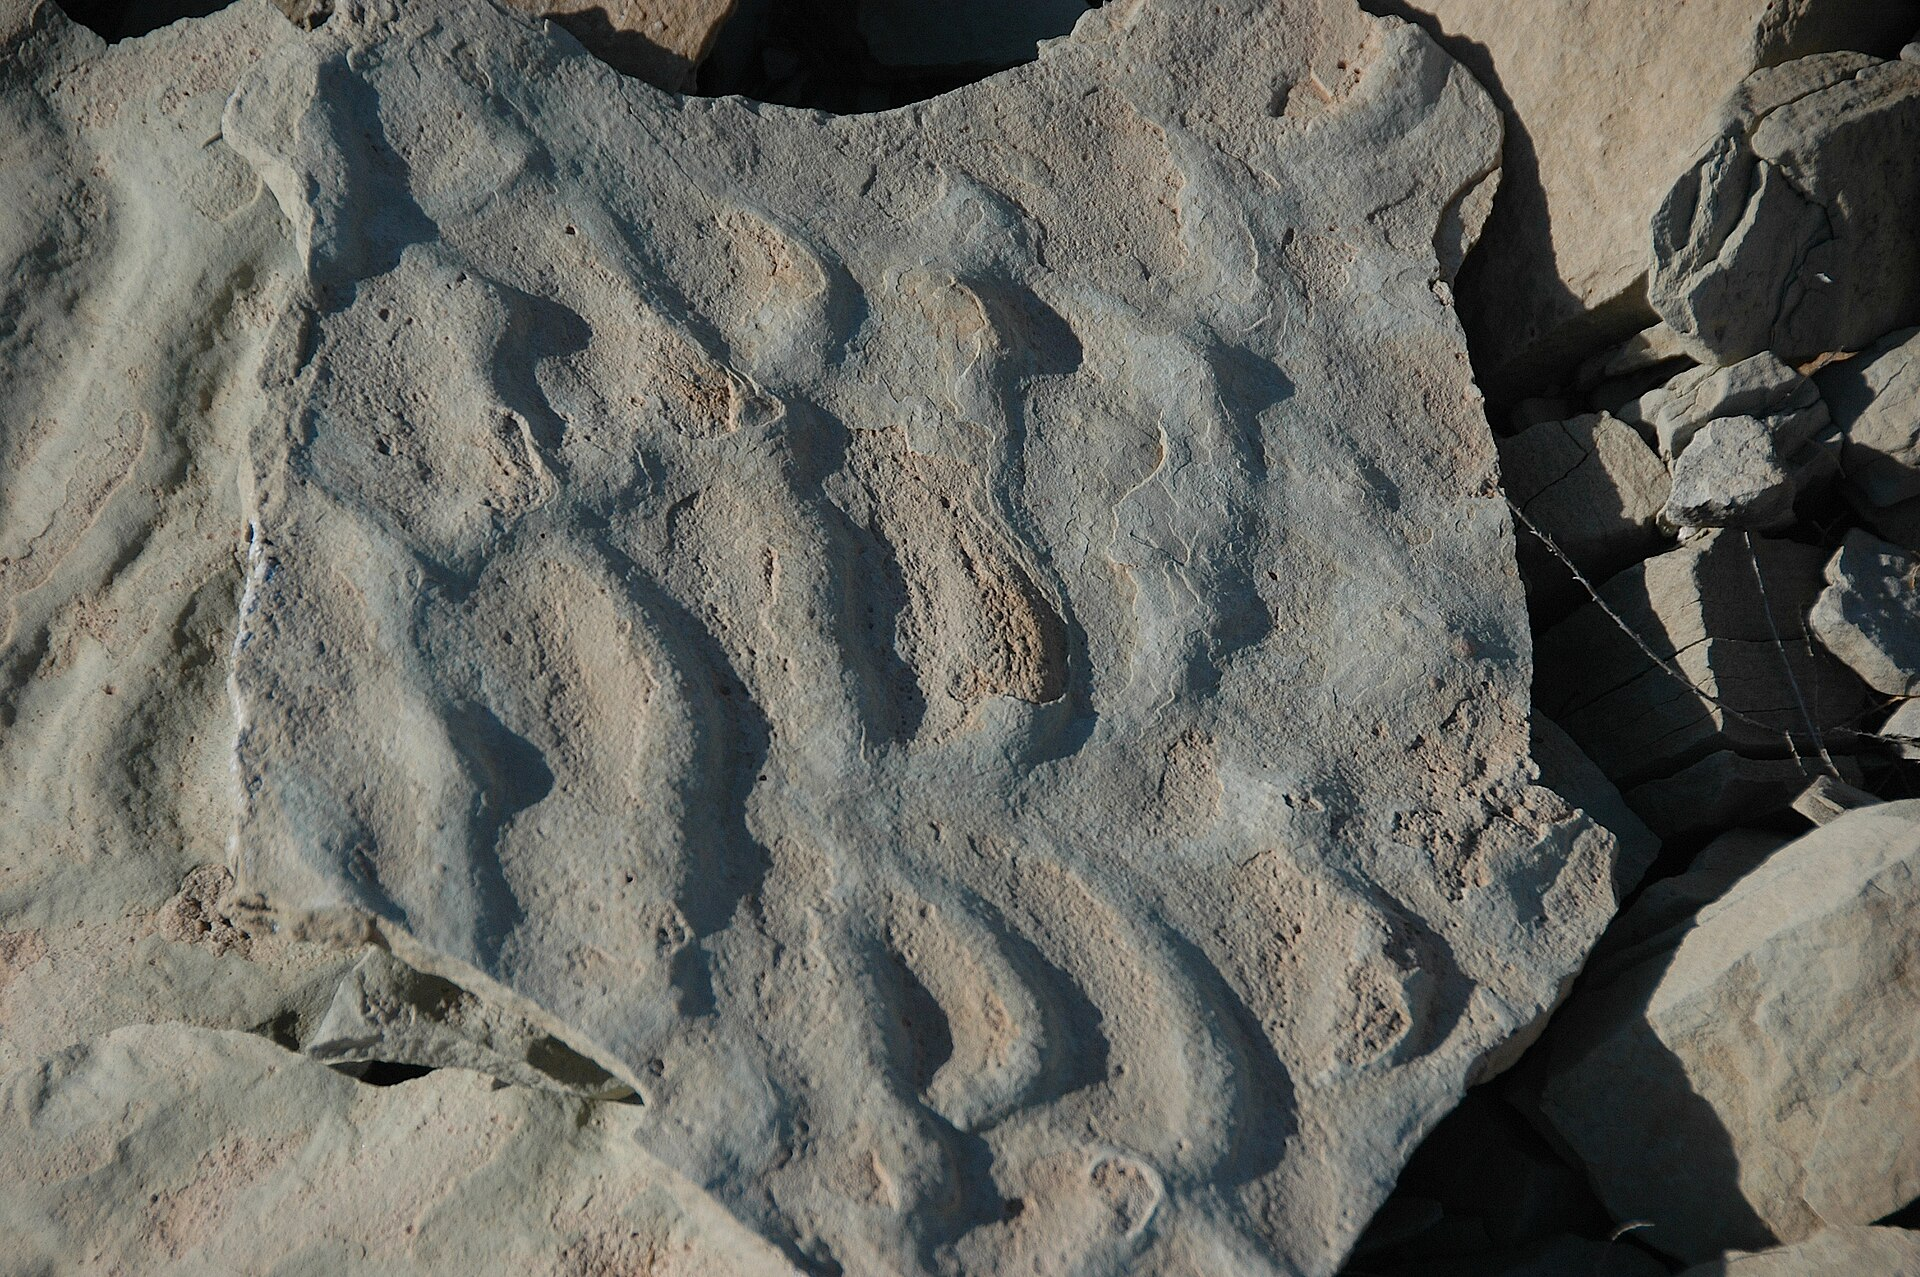
\includegraphics[width=0.56\linewidth]{images/book1/g7-ripple-marks.jpg}

{\small 砂岩板上的波痕，位于犹他州国会礁
国家公园（美国）：这些沙曾被流动的水激起波纹，
与今日海滩或溪床的沙相似。照片：James
St.~John（CC BY 2.0，经维基共享资源）。}
% ledger: commons:ripples, nps:ripple-marks
\label{fig:g7:sediments-and-fossils:ripples}
\end{omfigure}

\begin{example}[大峡谷的顶部]\label{ex:g7:sediments-and-fossils:kaibab}
凯巴布石灰岩是大峡谷顶部的一层，充满
腕足动物的壳和海百合的茎节，二者都是\omterm{def:g2:water-on-earth:ocean}{海洋}动物。它
形成于海底。如今同一岩层位于\omterm{def:g4:world-physical-map:altitude}{海平面}以上约
\qty{2700}{m}（\num{9000}~英尺）处：自其形成以来，
整个地区已被抬升。
% ledger: nps:grca-fossils, nps:grca-kaibab
\end{example}

一叠岩层可以画成\emph{\omterm{def:g7:sediments-and-fossils:layer}{地层}柱状图}：各岩层按
形成的先后顺序堆叠，厚度按比例绘出，其线索
标注于一侧。瓦尔登\omterm{def:g1:landscapes-around-us:landform}{丘陵}是本系列练习中虚构的地区，
其\omterm{def:g7:sediments-and-fossils:layer}{地层}柱状图如下。

\begin{omfigure}
\begin{tikzpicture}
  \begin{axis}[width=4.2cm, height=9.2cm, scale only axis=false, xmin=0, xmax=1, ymin=-60, ymax=485,
      axis x line=none, axis y line*=left, ytick={0,100,200,300,400},
      ylabel={距砂岩底部以上的高度（米）}, label style={font=\footnotesize},
      tick label style={font=\scriptsize}, clip=false]
    \addplot[lith schist, draw=black!70, line width=0.3pt] table {figdata/out/grade-7-varden_column-unit-older.dat};
    \addplot[lith sandstone, draw=black!70, line width=0.3pt] table {figdata/out/grade-7-varden_column-unit-sandstone.dat};
    \addplot[lith limestone, draw=black!70, line width=0.3pt] table {figdata/out/grade-7-varden_column-unit-limestone.dat};
    \addplot[lith shale, draw=black!70, line width=0.3pt] table {figdata/out/grade-7-varden_column-unit-shale.dat};
    \addplot[om lith={white}{om limestone}, draw=black!70, line width=0.3pt] table {figdata/out/grade-7-varden_column-unit-chalk.dat};
    \node[anchor=west, align=left, font=\footnotesize] at (axis cs:1.12,450) {\textbf{白垩}：顶部已被 \\剥蚀（仅画出底部）};
    \node[anchor=west, align=left, font=\footnotesize] at (axis cs:1.12,350) {\textbf{页岩}，\qty{100}{m}：颗粒极细；\\菊石};
    \node[anchor=west, align=left, font=\footnotesize] at (axis cs:1.12,210) {\textbf{石灰岩}，\qty{180}{m}：\\珊瑚与贝壳};
    \node[anchor=west, align=left, font=\footnotesize] at (axis cs:1.12,60) {\textbf{砂岩}，\qty{120}{m}：\\波痕、足迹};
    \node[anchor=west, align=left, font=\footnotesize] at (axis cs:1.12,-30) {更老的岩石（片岩和花岗岩），\\在砂岩到来之前已被磨平};
  \end{axis}
\end{tikzpicture}

\medskip
{\small 瓦尔登\omterm{def:g1:landscapes-around-us:landform}{丘陵}的\omterm{def:g7:sediments-and-fossils:layer}{地层}柱，是本系列中虚构的地区：
各岩层按形成先后排列，最早形成的在底部，
厚度按比例绘制。旁边标注的\omterm{def:g7:sediments-and-fossils:fossil}{化石}与痕迹
为练习数据。}
% ledger: (invented region: figdata/shared/region.py, drawn by figdata/grade-7/varden_column.py)
\label{fig:g7:sediments-and-fossils:column}
\end{omfigure}

\begin{omfigure}
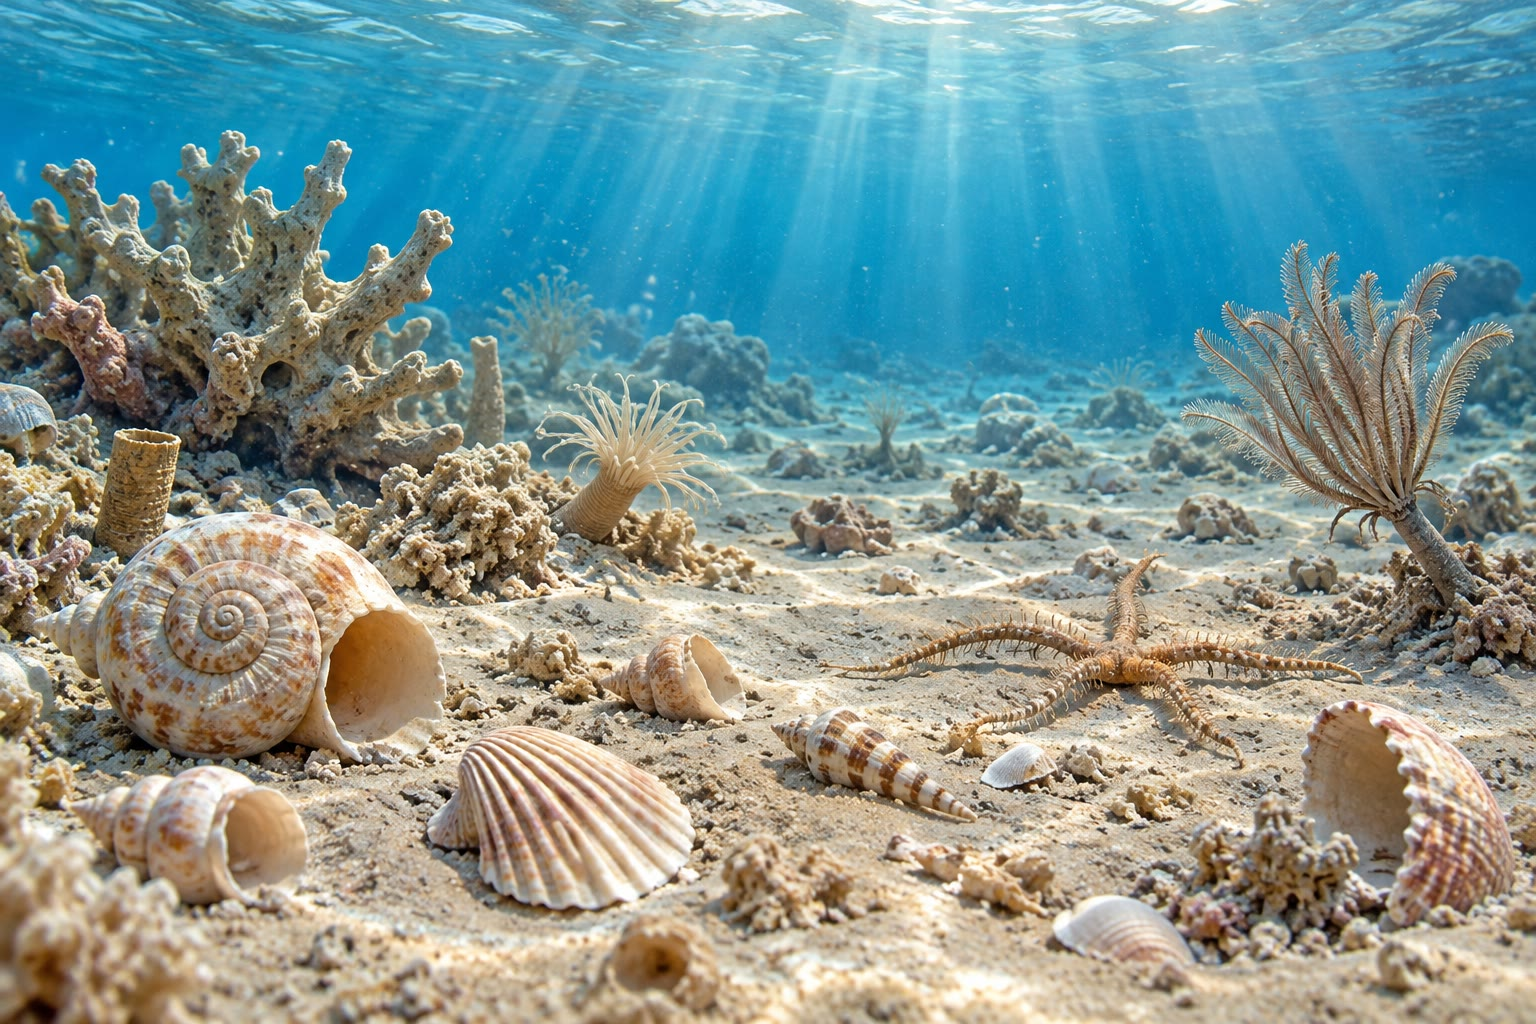
\includegraphics[width=0.6\linewidth]{images/book1/ai/g7-shallow-sea.jpg}

{\small 很久以前温暖浅海的海底，
大致是这样：贝壳与珊瑚碎片正在\omterm{def:g5:water-shapes-the-land:deposition}{沉积}，
将形成未来的石灰岩（AI 生成的通用场景示意图）。}
\label{fig:g7:sediments-and-fossils:shallow-sea}
\end{omfigure}

\begin{remark}[观察、拍照、留下]\label{rem:g7:sediments-and-fossils:leave}
在许多受保护的地区，禁止带走\omterm{def:g7:sediments-and-fossils:fossil}{化石}：例如在大峡谷，
挖掘、移动或带走任何\omterm{def:g7:sediments-and-fossils:fossil}{化石}都是违法的。
游客若发现\omterm{def:g7:sediments-and-fossils:fossil}{化石}，可拍照或画下来，
并将其留在原处，供他人观赏、供科学家研究，
并告知护林员。
\end{remark}
% ledger: nps:grca-fossils

\begin{inthefield}[正在形成的沉积物]
在海滩、湖岸或溪流岸边，与成人一起观察
浅水下的\omterm{def:g3:stones-pebbles-sand:sand}{沙子}：流动的水会把它冲成波纹，
与古老砂岩中保存的波纹相似。在湿沙近水边处留下一个脚印，
观察接下来的海浪会对它产生什么影响。
雨后，观察一个已干涸的水坑：坑底的沙上常覆盖一层薄薄的细泥——
最细的颗粒最后\omterm{def:g5:water-shapes-the-land:deposition}{沉积}，那时水还很平静。
画下所见，
并记下地点与时间。
\end{inthefield}
% ledger: nps:ripple-marks, ucmp:footprints, usgs:strata

\section{练习}

\begin{exercise}[$\star$]\label{exo:g7:sediments-and-fossils:1}
请将每个词与其含义配对：\omterm{def:g7:sediments-and-fossils:sediment}{沉积物}、\omterm{def:g7:sediments-and-fossils:layer}{地层}、\omterm{def:g7:sediments-and-fossils:fossil}{化石}、\omterm{def:g7:sediments-and-fossils:fossil}{外模}、
\omterm{def:g7:sediments-and-fossils:fossil}{内模}、\omterm{def:g7:sediments-and-fossils:fossil}{遗迹化石}。(a) \omterm{def:g3:stones-pebbles-sand:rock}{岩石}中因贝壳溶解而留下的空穴。
溶解。(b) 保存在\omterm{def:g3:stones-pebbles-sand:rock}{岩石}中的足迹或洞穴。(c) 由水、风或冰
堆积的松散物质。(d) 空穴被\omterm{def:g6:rocks-and-minerals:mineral}{矿物}充填后形成的石质复制品。
(e) 同时形成的一层\omterm{def:g7:sediments-and-fossils:sediment}{沉积物}。(f)
很久以前生物的遗体或遗迹，保存于\omterm{def:g3:stones-pebbles-sand:rock}{岩石}中。
\end{exercise}

\begin{exercise}[$\star$]\label{exo:g7:sediments-and-fossils:2}
将下列步骤按顺序排列，说明贝壳如何
在地表变为\omterm{def:g7:sediments-and-fossils:fossil}{化石}：(a) \omterm{def:g5:water-shapes-the-land:erosion}{侵蚀}作用剥去其上方的岩层；(b) 动物
死于海底；(c) 新的岩层不断堆积，贝壳变为石头；
(d) 泥很快覆盖了贝壳。
\end{exercise}

\begin{exercise}[$\star$]\label{exo:g7:sediments-and-fossils:3}
利用线索表，判断每一层形成于何处。(a) 布满珊瑚的
石灰岩。(b) 表面有波痕的砂岩。(c) 一层黑色的
煤层。(d) 带有叶的印痕和蜻蜓翅膀的页岩。
\end{exercise}

\begin{exercise}[$\star$]\label{exo:g7:sediments-and-fossils:4}
判断下列说法正误，并改正错误的说法。(a) 每一只死去的动物
终将变成\omterm{def:g7:sediments-and-fossils:fossil}{化石}。(b) 足迹可以是\omterm{def:g7:sediments-and-fossils:fossil}{化石}。(c) 浑浊的水
流变慢时，细泥最先沉降。(d) \omterm{def:g7:sediments-and-fossils:sediment}{沉积物}是
水平铺展\omterm{def:g5:water-shapes-the-land:deposition}{沉积}而成的。
\end{exercise}

\begin{exercise}[$\star\star$]\label{exo:g7:sediments-and-fossils:5}
利用瓦尔登\omterm{def:g1:landscapes-around-us:landform}{丘陵}的\omterm{def:g7:sediments-and-fossils:layer}{地层}柱。(a) 给出砂岩、
石灰岩和页岩的厚度。(b) 它们的总厚度是多少？
(c) 石灰岩占这一总厚度的百分之几？结果
取最接近的整数。(d) 为什么\omterm{def:g7:sediments-and-fossils:layer}{地层}柱没有给出
白垩的厚度？
\end{exercise}

\begin{exercise}[$\star\star$]\label{exo:g7:sediments-and-fossils:6}
一名学生摇晃装有水、\omterm{def:g3:stones-pebbles-sand:pebble}{砾石}、沙和泥的罐子，
让其静置。(a) 第二天画出罐子，并标注各层。(b) 为何
一小时后水仍然浑浊？(c) 她再次加入沙和泥并
静置。现在罐底看到的是什么？(d) 罐中哪一层
最先形成？
\end{exercise}

\begin{exercise}[$\star\star$]\label{exo:g7:sediments-and-fossils:7}
下列哪一项最有可能形成\omterm{def:g7:sediments-and-fossils:fossil}{化石}，哪一项最不可能？
请说明理由。(a) 被冲上\omterm{def:g3:stones-pebbles-sand:rock}{岩石}\omterm{def:g1:landscapes-around-us:water}{海岸}的水母。(b) 一枚
埋在平静\omterm{def:g1:landscapes-around-us:water}{湖泊}\omterm{def:g3:stones-pebbles-sand:sand}{淤泥}中的蜗牛壳。(c) 多年躺在干燥\omterm{def:g1:landscapes-around-us:landform}{平原}
上的骨头。(d) \omterm{def:g1:landscapes-around-us:water}{河流}\omterm{def:g5:water-shapes-the-land:flood}{洪水}时被沙覆盖的蛤壳。
\end{exercise}

\begin{exercise}[$\star\star$]\label{exo:g7:sediments-and-fossils:8}
一枚贝壳被埋在沙中，沙后来变成砂岩。渗过\omterm{def:g3:stones-pebbles-sand:rock}{岩石}的水
将贝壳完全溶解。(a) \omterm{def:g3:stones-pebbles-sand:rock}{岩石}中还留下什么？(b) 之后，\omterm{def:g6:rocks-and-minerals:mineral}{矿物}
充满了这一空穴，会形成什么？(c) 贝壳本身是否
仍然存在？(d) 为什么\omterm{def:g7:sediments-and-fossils:fossil}{外模}和\omterm{def:g7:sediments-and-fossils:fossil}{内模}在砂岩中
比在页岩中更常见？（想一想：水在颗粒之间穿过有多容易。）
\end{exercise}

\begin{exercise}[$\star\star$]\label{exo:g7:sediments-and-fossils:9}
大峡谷的平均深度为 \qty{1.6}{km}。(a) 将这一深度
换算为米。(b) 设峡谷两壁由每层厚 \qty{80}{m} 的岩层组成，
从峡谷边缘到谷底能容纳多少层？(c) 厚 \qty{160}{m}
的一层占深度的百分之几？
\end{exercise}

\begin{exercise}[$\star\star$]\label{exo:g7:sediments-and-fossils:10}
在一层砂岩中发现了恐龙足迹。(a) 恐龙是否
在坚硬的\omterm{def:g3:stones-pebbles-sand:rock}{岩石}上行走？请说明理由。(b) 为何
留在泥质岸边的大多数足迹会消失？(c) 恐龙经过之后不久，
必须发生什么，足迹才能被保存？(d) 足迹属于
实体\omterm{def:g7:sediments-and-fossils:fossil}{化石}还是\omterm{def:g7:sediments-and-fossils:fossil}{遗迹化石}？
\end{exercise}

\begin{exercise}[$\star\star\star$]\label{exo:g7:sediments-and-fossils:11}
在\omterm{def:g1:landscapes-around-us:water}{湖泊}中，每次\omterm{def:g5:water-shapes-the-land:flood}{洪水}都会留下一层约 \qty{2}{cm} 厚的沙，
\omterm{def:g5:water-shapes-the-land:flood}{洪水}过后的平静数周则留下一层约 \qty{5}{mm} 厚的泥，
（练习数据）。(a) 一对层的厚度是多少毫米？
(b) 从湖底取出的一根岩芯长 \qty{1}{m}，且仅由
这样的层对组成。它记录了多少次\omterm{def:g5:water-shapes-the-land:flood}{洪水}？(c) 靠近\omterm{def:g5:water-shapes-the-land:source-mouth}{河口}处的
沙层较厚，远离\omterm{def:g5:water-shapes-the-land:source-mouth}{河口}处的沙层较薄。请解释原因。(d) 为何
远离\omterm{def:g5:water-shapes-the-land:source-mouth}{河口}处的泥比沙多？
\end{exercise}

\begin{exercise}[$\star\star\star$]\label{exo:g7:sediments-and-fossils:12}
\omterm{def:g3:stones-pebbles-sand:rock}{岩石}中发现的\omterm{def:g7:sediments-and-fossils:fossil}{化石}大多是贝壳和微小的遗骸；\omterm{def:g7:sediments-and-fossils:fossil}{化石}
中软体动物的\omterm{def:g7:sediments-and-fossils:fossil}{化石}很少，恐龙在全部\omterm{def:g7:sediments-and-fossils:fossil}{化石}中只占极小的一部分。
(a) 解释为何贝壳如此常见。(b) 解释为何软体
动物很少见。(c) 一位科学家想知道古代\omterm{def:g2:water-on-earth:ocean}{海洋}中生活过的全部动物。
\omterm{def:g7:sediments-and-fossils:fossil}{化石}能否给出完整的名单？请说明理由。
\end{exercise}

\section{问题：瓦尔登丘陵的地层柱}

\begin{problem}[{周末问题——逐层读取瓦尔登丘陵的岩层，
根据化石判断它们形成的地点，并算出
堆积石灰岩所需的时间}]
\label{pb:g7:sediments-and-fossils:1}
% ledger: (invented region: figdata/shared/region.py; rates are exercise data, figdata/grade-7/varden_column.py part rates)
利用本章中瓦尔登\omterm{def:g1:landscapes-around-us:landform}{丘陵}的\omterm{def:g7:sediments-and-fossils:layer}{地层}柱。其砂岩中
有波痕和足迹；其石灰岩中有珊瑚和贝壳；其
页岩由极细的颗粒组成，并含有菊石；顶部的白垩
已被部分\omterm{def:g5:water-shapes-the-land:erosion}{侵蚀}。

\medskip
\noindent\textbf{第一部分——读取岩层。}\par\nopagebreak
\begin{enumerate}[beginpenalty=10000]
  \item 列出这四层岩层，从最先\omterm{def:g5:water-shapes-the-land:deposition}{沉积}的一层到最后一层。
  \item 给出砂岩、石灰岩和页岩的厚度，
        以及它们的总厚度。
  \item 石灰岩占这一总厚度的百分之几？
  \item 为何没有人能说出白垩在形成时有多厚？
\end{enumerate}

\medskip
\noindent\textbf{第二部分——其中的\omterm{def:g7:sediments-and-fossils:fossil}{化石}。}\par\nopagebreak
\begin{enumerate}[resume, beginpenalty=10000]
  \item 砂岩形成于何处？给出两条线索。
  \item 石灰岩形成于何处？给出一条线索。
  \item 页岩由极细的颗粒组成。\omterm{def:g5:water-shapes-the-land:deposition}{沉积}时水体是平静的还是流动的？
        请说明理由。
  \item 用三句话讲述这一地点的故事，从砂岩
        到页岩。
\end{enumerate}

\medskip
\noindent\textbf{第三部分——所用时间。}\par\nopagebreak
\begin{enumerate}[resume, beginpenalty=10000]
  \item 以厘米为单位写出石灰岩的厚度。
  \item 假设砂岩每 20 年堆积 \qty{1}{cm}。其 \qty{120}{m} 厚的砂岩
        用了多少年？
  \item 假设石灰岩每 100 年堆积 \qty{1}{cm}。
        \qty{1}{m} 厚的石灰岩用了多少年？
  \item \qty{180}{m} 厚的石灰岩用了多少年？这比
        砂岩所用的时间长多少倍？
\end{enumerate}
\end{problem}
